\chapter{Background}
The following chapter provides the basic high-level background knowledge necessary for understanding the subsequent chapters and also defines the important terminology that is relevant for our work.

\section{OSI Model and Network Layers}
In order for the devices from all over the world to properly communicate and exchange data there is a necessity for communication models. The official standardized version of such models is the \acl{osi}(OSI) model, developed by \acl{iso}\cite{osi_iso}. It consists of 7 layers each of them having a specific purpose. However OSI model is only conceptual and it differs from the architectures that are actually used by networks. One of such architectures is Internet Protocol Suite, also known as TCP/IP. The figure \ref{osi_tcp_ip} visualizes the layers of both of these models.

\begin{figure}[H]
 \centering
 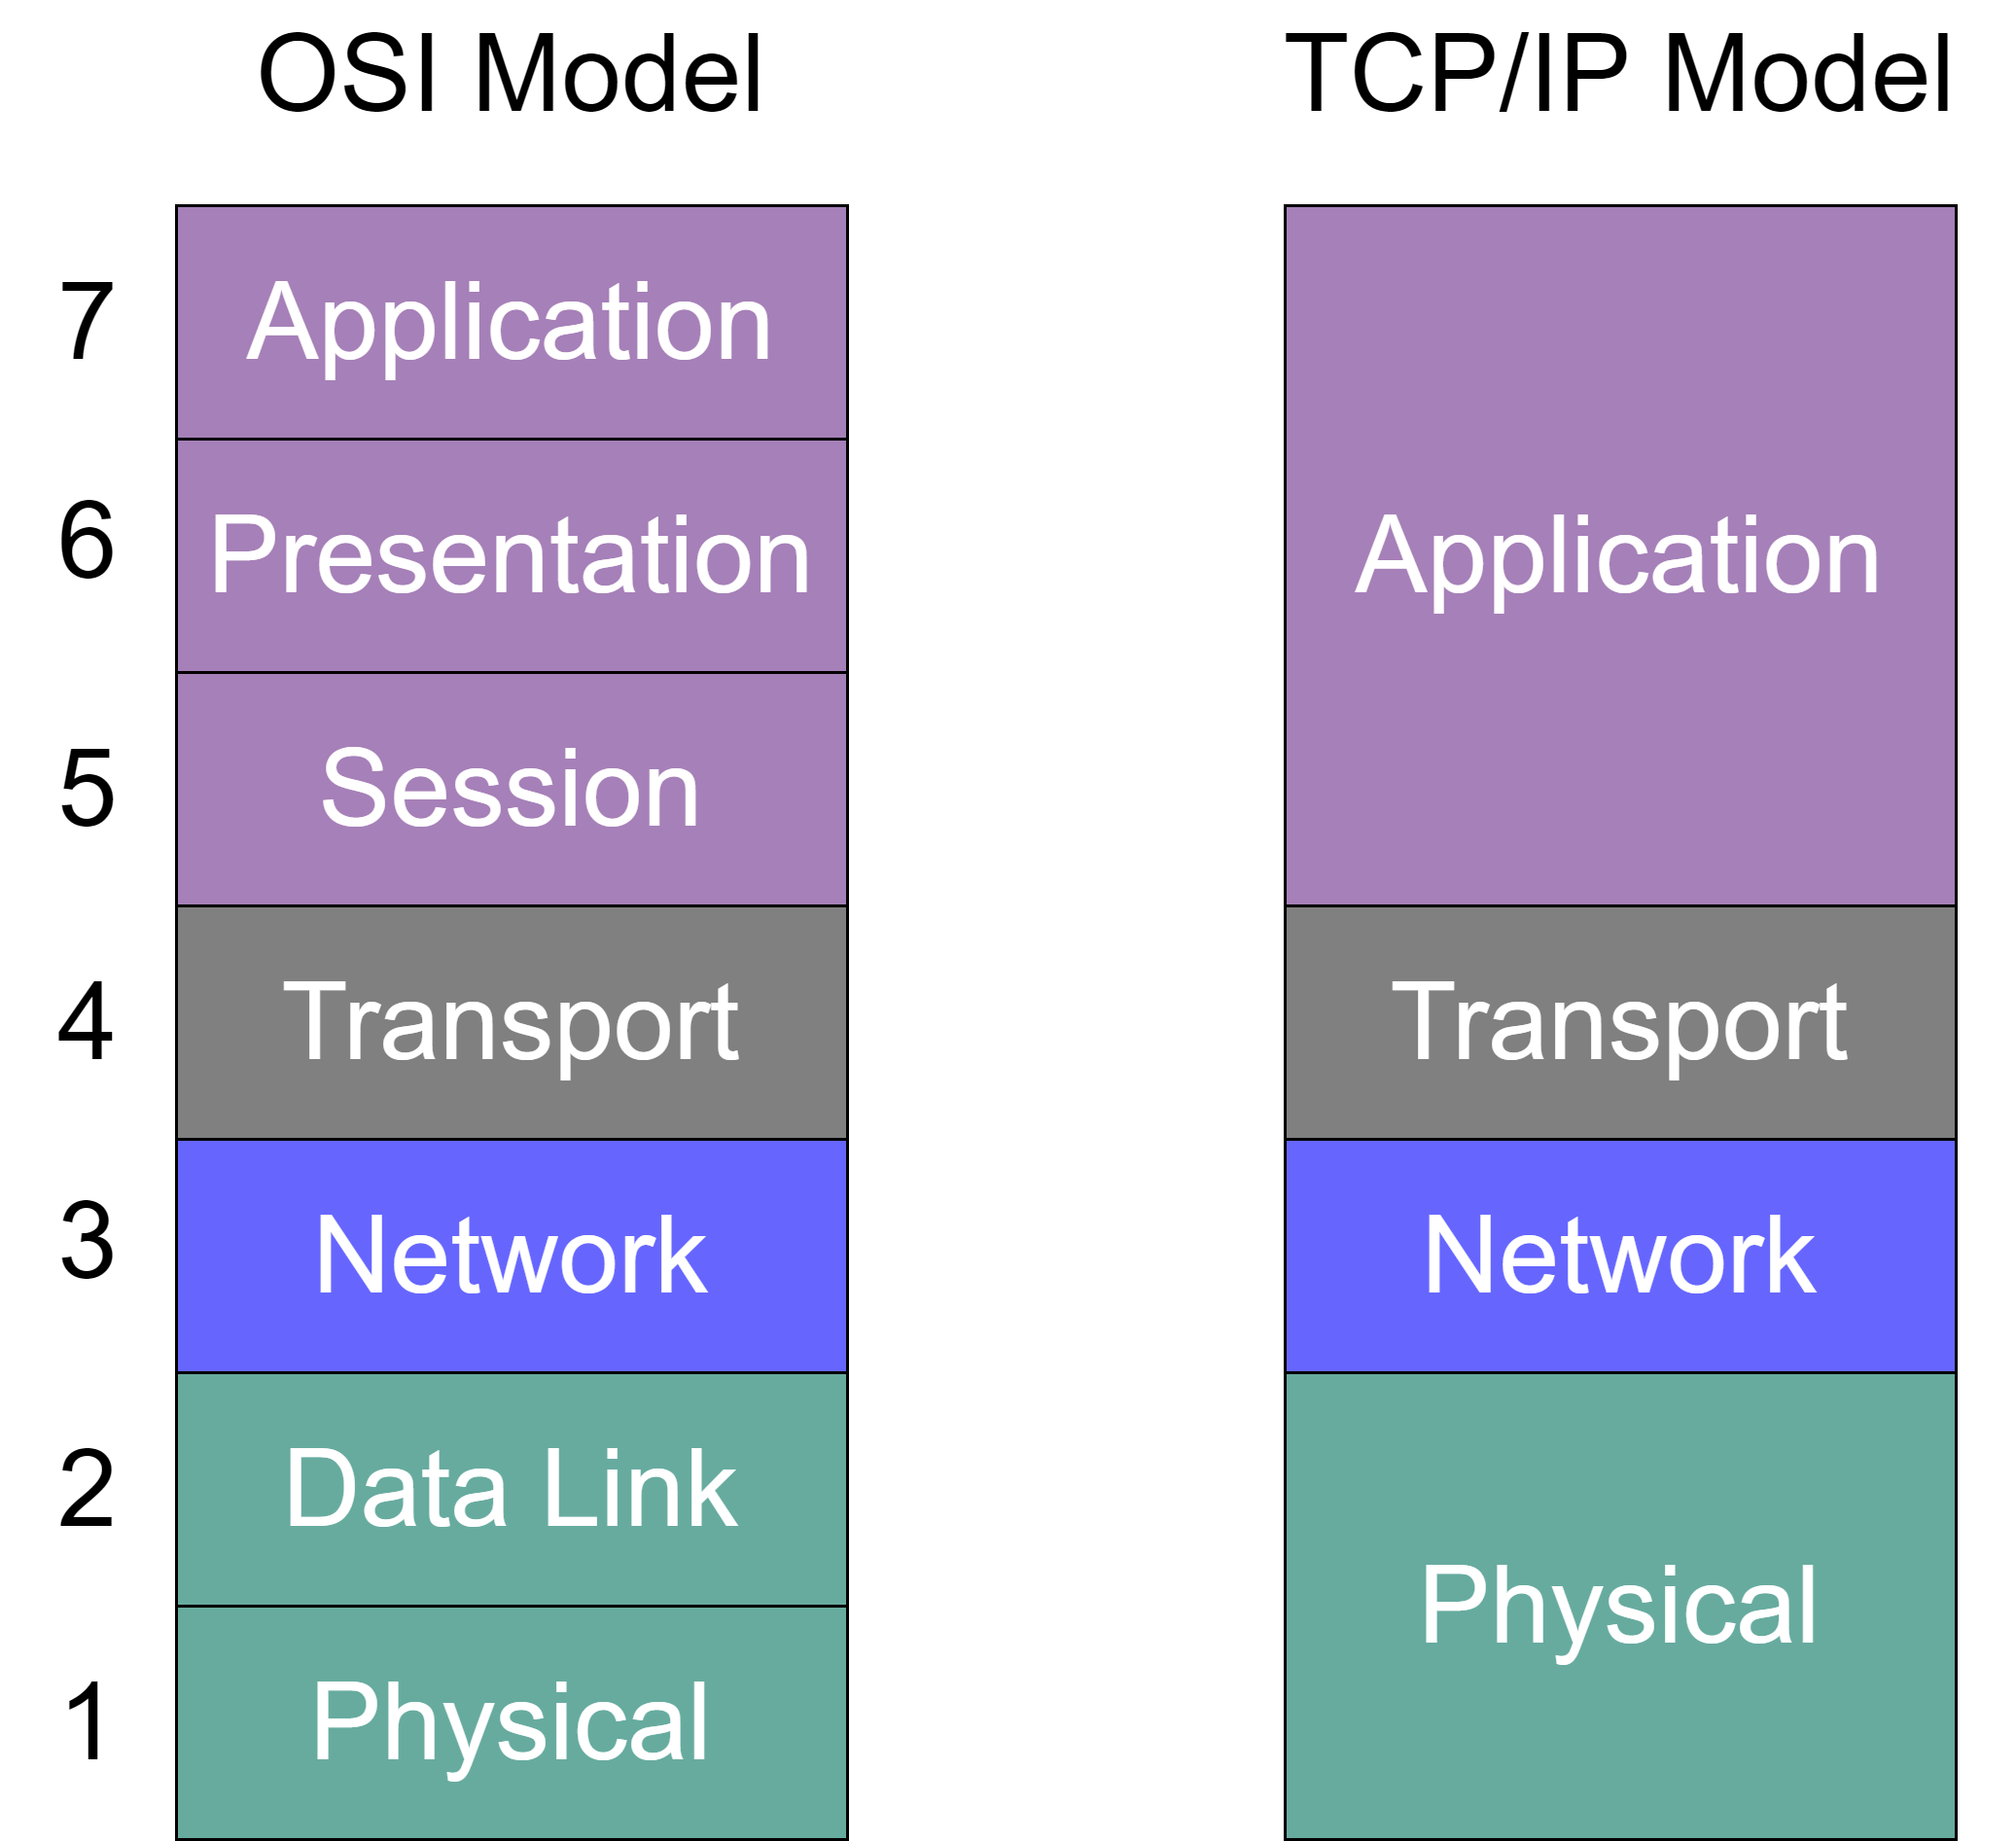
\includegraphics[width=0.7\textwidth]{layers.png}
 \caption{Comparison of OSI and TCP/IP Models}
 \label{osi_tcp_ip}
\end{figure}

We will shortly describe each OSI layer as defined in "Networking - the Complete Reference"\cite{osi_model_ref}.
\begin{itemize}
	\item The Physical and Data Link layers are responsible for the physical communications between devices, i.e. transporting data bits from one machine to another. 
	\item The Network layer functions as a carrier of messages from the source system to the final destination. It provides end-to-end addressing, routing and error checking.
	\item The Transport layer takes care of packet segmentation and reassembling once they reach the destination. Port numbers are specified at this layer. 
	\item The Session, Application and Presentation layers are used for user interaction through software applications.
\end{itemize}

Sending data in the Internet is operated from top down through these layers and receiving goes bottom up.

The scope of this thesis are the transport and the network layers and the protocols that we are focusing on are \acl{ip}(IP) and \acl{icmp}(ICMP) from the Network layer  and \acl{tcp} and \acl{udp} from the Transport layer.\\
We will further refer to the Transport layer as layer 4 (L4) and the Network layer as layer 3 (L3).

\section{Network Layer Protocols}
\subsection{Internet Protocol (IP)}
\label{ip_descr}
For the elaboration about L3 and L4 protocols we will use the definitions by Internet Engineering Task Force (IETF)\cite{ietf_ip}.

As mentioned above, the Layer 3 is responsible for end-to-end addressing and routing. The most common L3 protocol is IP. 
The IP protocol transports the data packets from one host to another and in order to accomplish this goal it encapsulates TCP or UDP packets provided by the Transport layer. 
The figure \ref{ip_header}\cite{iph} represents the structure of IP packet headers.

\begin{figure}[H]
 \centering
 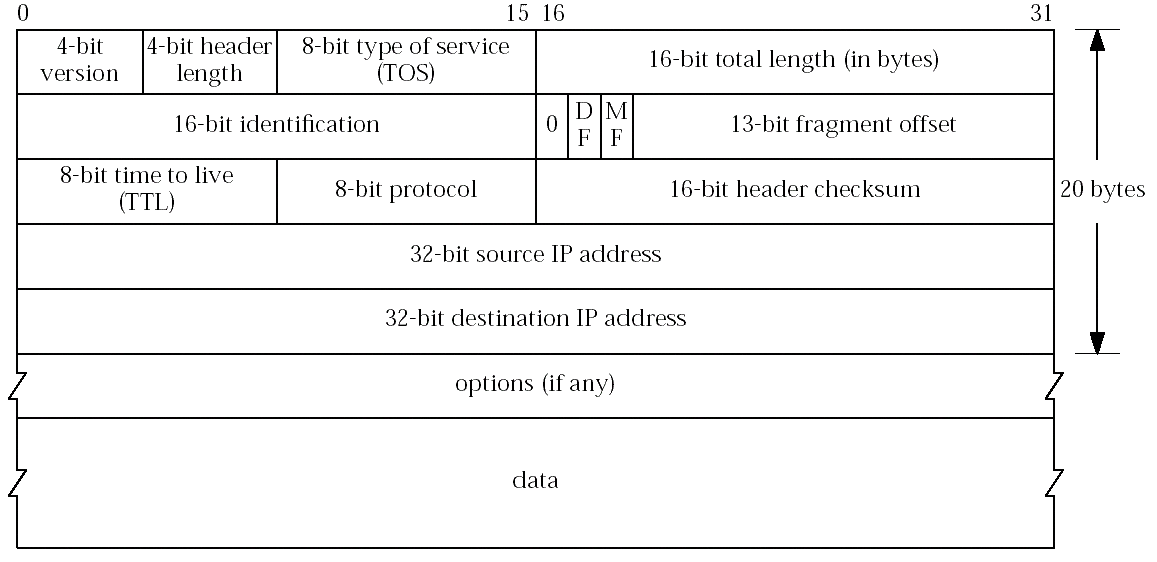
\includegraphics[width=\textwidth]{ipheader.png}
 \caption{Structure of IP header}
 \label{ip_header}
\end{figure}

As it can be seen, there is an 8-bit time to live (TTL) field in the IP header. It is implemented to control the maximum time that a packet is allowed to stay in a network. This is necessary in order to avoid the looping of a packet between hosts. Each IP packet is assigned a certain TTL value and it decrements after each router that a packet passes through. If a packet is unable to reach the final destination before ttl equals zero it will be discarded and an error message will be returned to the sender.\\
This thesis is built upon taking advantage of this functionality to use it for accomplishing our goal.


\subsection{Internet Control Message Protocol (ICMP)}
\label{icmp_section}
Another Network layer protocol that is crucial for our work is \sc{icmp}. 
It is used for delivering control messages back to the sender whenever a problem arises in a network\cite{ietf_icmp}. As there exits a multitude of types of problems in the Internet ICMP packet header contains a Type field to classify the issues for the sender. 
The table \ref{icmp_types} provides the incomplete list of ICMP message types.

\begin{table}[H]
\centering
\begin{tabular}{ | m{3cm} | m{5cm}| } 
  \hline
	Message type & Description \\
  \hline
    0 & Echo Reply  \\
    3 & Destination Unreachable \\
    4 & Source Quench \\
    5 & Redirect \\
    8 & Echo Request \\
    11 & Time Exceeded \\
    12 & Parameter Problem \\
    13 & Timestamp Request \\
    14 & Timestamp Reply \\
    15 & Info Request \\
    16 & Info Reply \\
    17 & Address Mask Request \\
    18 & Address Mask Reply \\ 
  \hline
\end{tabular}
\caption{ICMP message types \cite{icmp_man}}
\label{icmp_types}
\end{table}

Our object of interest are type 11 time exceeded ICMP messages. This is the type that provides feedback when the TTL field of an IP address reaches the value of 0.\\
We will describe how we use this feature in more detail in the Implementation section.

\section{Transport Layer Protocols}

\subsection{Transmission Control Protocol (TCP)}
\acl{tcp} serves as a highly reliable data transfer protocol which guarantees that all the packets sent from the source host will reach the destination. It is used in services where the reliability is a requirement, e.g. sending emails or transferring files.\\
This reliability is provided by the connection establishment process called three-way handshake. 
During this process the source host sends a packet with a \texttt{SYN} synchronization flag and the destination host responds with a packet with an \texttt{ACK} acknowledgement flag. In turn the first host also returns a packet with an \texttt{ACK} flag. Once the connection is established the source can send more packets to the end host. 

To further ensure the reliability, the sender host requires an \texttt{ACK} signal for every packet it sends. For this it assigns each packet a sequence number and expects a corresponding acknowledgement for each such packet. If the \texttt{ACK} signals are not received, packets with respective sequence numbers are sent again\cite{ietf_tcp}.



\subsection{User Datagram Protocol (UDP)}
Another famous Transport layer protocol is the \acl{udp}. Unlike TCP, which is known for its reliability, UDP is less reliable. But on the other hand it is aiming to transfer data from one host to another with minimal protocol mechanism\cite{ietf_udp}\\
UDP is used in situations where the certain rate of packet loss can be tolerated, such as video streaming. 



\section{Terminology}
Certain terminology in our field of research can be used with different meanings, therefore we first need to state that this thesis will be using the definitions provided by Prasad et al in their paper "Bandwidth estimation: metrics, measurement, techniques and tools"\cite{Prasad2003}, as it appears to be more widespread and accepted. Moreover, those are the definitions also used by other researchers at the chair, therefore, it is more practical to use the common language.

Prasad et al\cite{Prasad2003} introduce the following three metrics: capacity, bandwidth and bulk transfer capacity(BTC) and capacity is the primary focus of our work.
Moreover, they distinguish between segments and hops. The former being the link at the data link layer (L2) and the latter - the links at the IP layer (L3). 

Furthermore, they define segments as physical links between devices or shared access local area networks, while hops as sequences of one or more segments connected through Layer 2 devices. Additionally they define end-to-end path from a source host to a destination host as a sequence of hops.


\subsection*{Capacity}
Prasad et al. define the capacity $C_i$ of a hop $i$ as a maximum possible amount of bits that can be transferred at that hop per second\cite{Prasad2003}. If a path consists of several hops, the capacity of the whole path equals that of the link with the lowest capacity:

\[C_{min}= \min_{i=1,..,n} C_i\] 

$C_{min}$ is referred as a narrow link. Prasad et al.\cite{Prasad2003} specify that they avoid the term "bottleneck" as it is interchangeably used for both minimal capacity and minimal available bandwidth, however we will use "bottleneck" to denote narrow link in this thesis.

%\Delta _{L3} = \dfrac{L_{L3}+H_{L2}}{C_{L2}}


\begin{figure}[H]
 \centering
 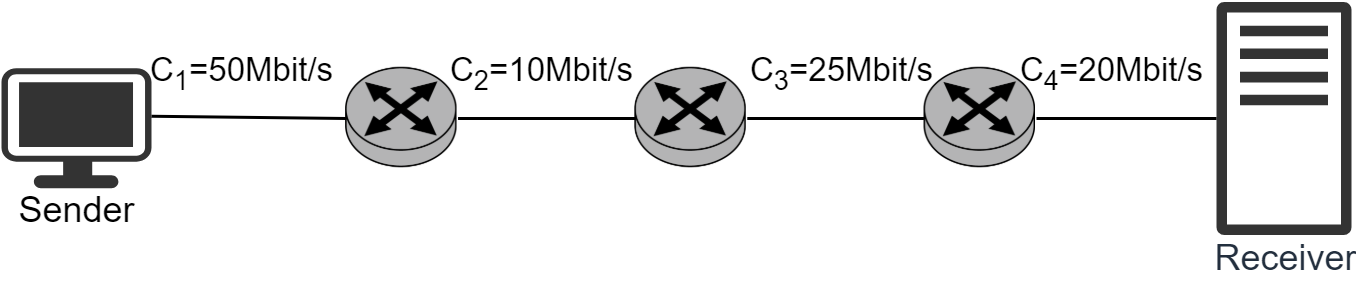
\includegraphics[width=\textwidth]{capacity_def.png}
 \caption{Sample network path and link capacities}
 \label{capacity_def}
\end{figure}

The figure \ref{capacity_def} presents a sample network path with four hops and the second hop $C_2$ as a bottleneck. The end-to-end capacity of this path will equal that of $C_2$, i.e. 10 Mbit/s


\subsection*{Available Bandwidth}
When working with network capacities it is also very important to understand the concept of available bandwidth of a link. Unlike capacity it is not a constant value and it refers to the unused, unconsumed capacity of a link at a certain moment of time\cite{Prasad2003}. 

\section{Traffic Generation}
Throughout our work it will be required to artificially generate traffic between hosts in a network and subsequently capture and analyze it. In this section we will briefly tackle several tools and methodologies that will be later used to achieve our goals.

\subsection*{Raw Sockets}
Network socket is the software used for data traffic between the hosts. 
A TCP packet consists of an IP header, a TCP header and a chunk of data it is supposed to deliver to another host\cite{tcp_raw_sockets}.\\
The default type of sockets has TCP and IP headers automatically added, however in certain cases, including our research, it is necessary to configure the headers manually with an application. In such cases raw sockets have to be used.\\
In this thesis we use raw sockets for traffic generation as it provides the ability to manipulate the \texttt{time to live} field of IP header, which will show to be a crucial part for our research.


\subsection*{iPerf}
Another powerful tool used in this thesis is iPerf\cite{iperf}. It is mainly used for the maximum achievable bandwidth estimation in IP networks, however it incorporates multitude of other features.\\
We will be using this tool for additional packet generation to emulate the cross-traffic in our test environment.

